%%%%%%%%%%%%%%%%%%%%%%%%%%%%%%%%%%%%%%%%%
% Full Length Professional CV
% LaTeX Template
% Version 2.0 (13/6/20)
%
% Original author:
% Sreedhar Unnikrishnakurup 
%
% Important note:
% This template requires the my_cv.cls file to be in the same directory as the .tex file. The my_cv.cls file provides the resume style used for structuring the document. THe publication.bib file is needed for adding the publication list
%
%%%%%%%%%%%%%%%%%%%%%%%%%%%%%%%%%%%%%%%%%

%----------------------------------------------------------------------------------------
%	PACKAGES AND OTHER DOCUMENT CONFIGURATIONS
%----------------------------------------------------------------------------------------

\documentclass{my_cv}% Use the custom my_cv.cls style
\begin{document}
\title{CV}
\author{Sreedhar Unnikrishnakurup}
\begin{minipage}{0.8\textwidth}
\begingroup
\let\center\flushleft
\let\endcenter\endflushleft
\maketitle
\endgroup
\end{minipage}
\begin{minipage}{0.1\textwidth}
\begin{tikzpicture}[remember picture,overlay]
\clip ($(current page text area.north east)!0.01!(current page text area.south east)!-7.4!(current page text area.north west)$)
  circle (2.1cm) node {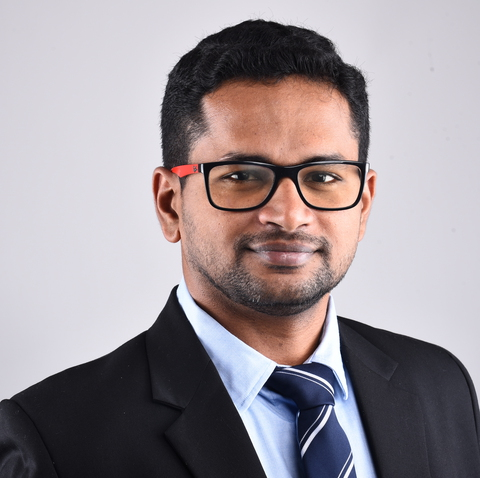
\includegraphics[width=2.3\linewidth]{mypic2}};
\end{tikzpicture}
%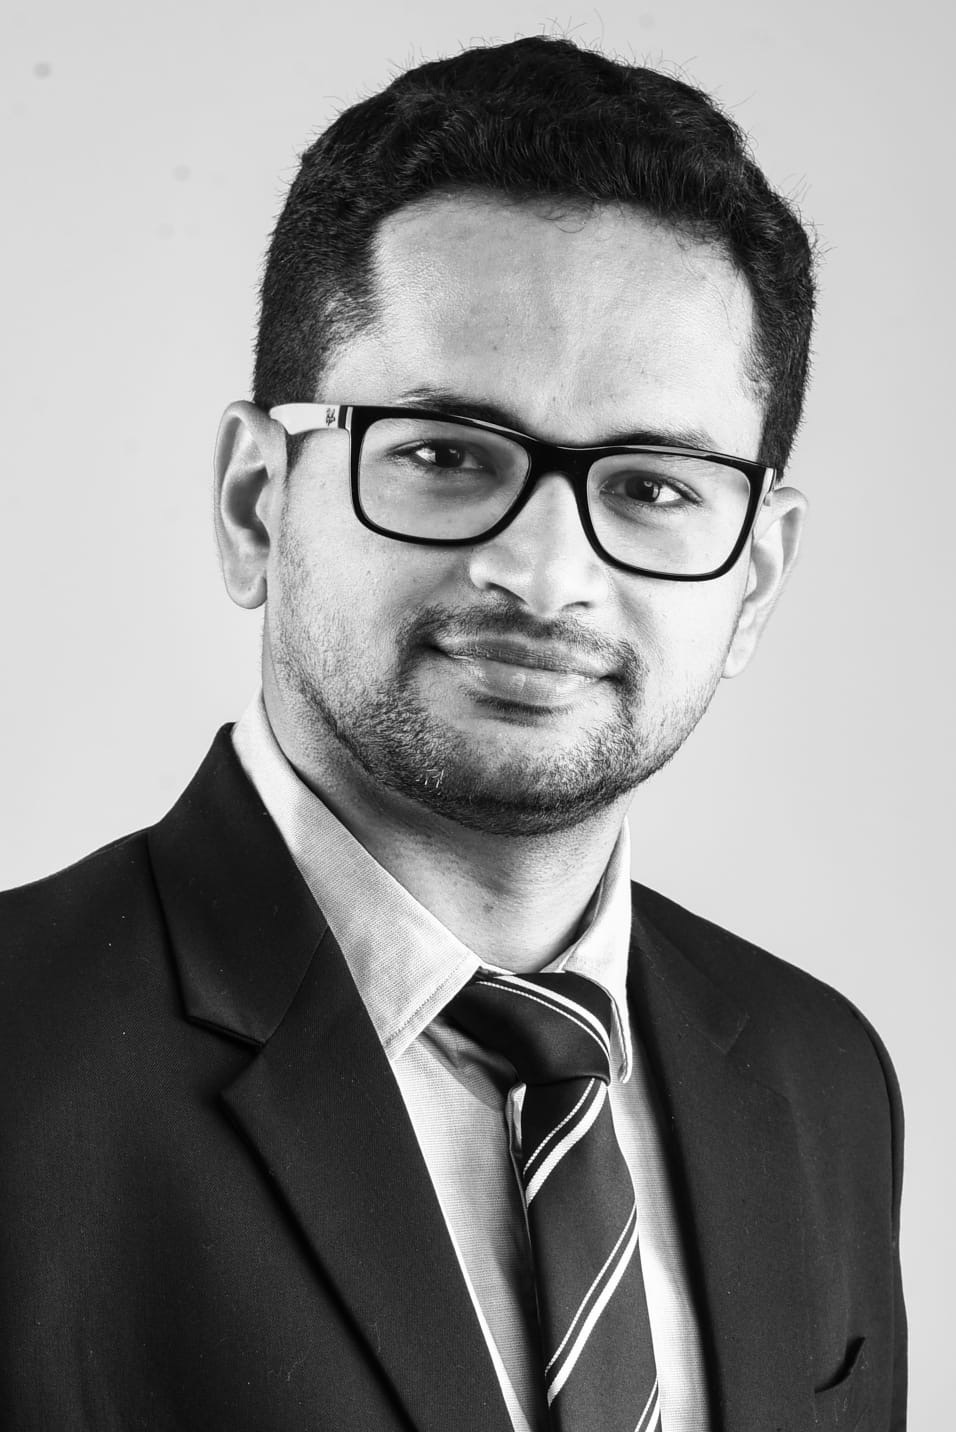
\includegraphics[width=8em]{mypic}
\end{minipage}
\vspace{1.5em}
%-------------------------------------------------------------
%	WORK EXPERIENCE SECTION
%-------------------------------------------------------------
\section{Work Experience}
\vspace{1.0em}
\subsection{Senior Project Officer}
\subsubsection{Centre for Non-Destructive Evaluation (CNDE), IIT Madras}
\datedsubsection{May 2018--Ongoing}{Chennai, India}
%\paragraph{
\begin{itemize}[leftmargin=0.15in]
\setlength\itemsep{-0.1em}
\color{mygray}
\item Application of Nondestructive evaluation techniques and deep learning models for thickness inspection of thermal barrier coatings
\item Online monitoring of CMT welding process for defect detection using infrared thermal imaging
\item Online inspection of cracks in continuous cast steel billets using infrared thermography
\item Development of artificial intelligence assisted advanced radiography imaging and automatic defect recognition of critical welds in ship industry
\end{itemize}%}
{\color{mygray1} \hdashrule[0.1ex]{18.8cm}{0.2mm}{1mm}}
%{\color{mygray} \rule{\linewidth}{0.5mm} }
\subsection{Cohort Member BA3}
\subsubsection{Entrepreneur First}
\datedsubsection{February 2020 - May 2020}{Bangalore, India}
\begin{itemize}[leftmargin=0.15in]
\setlength\itemsep{-0.1em}
\color{mygray}
\item Explored several interesting technological solutions, exploring the market, validating the technology, speaking to customers, and researching prototypes
\item The ideas that we worked on are detect and report quality-compromised and counterfeit drugs using a mobile cloud-based cost-effective hyper-spectral Imaging based AI device
\end{itemize}
{\color{mygray1} \hdashrule[0.1ex]{18.8cm}{0.2mm}{1mm}}
\subsection{Postdoctoral Research Scientist}
\subsubsection{NDT group 8.7, Federal Institute for Material Research and Testing (BAM)}
\datedsubsection{January 2016 - June 2017}{Berlin, Germany}
\begin{itemize}[leftmargin=0.15in]
\setlength\itemsep{-0.1em}
\color{mygray}
\item European Metrology Research Programme (EMRP) Validated Inspection Techniques for Composites in Energy applications (Collaborative project between institutes from UK, France, Germany and Czech Republic)
\item Development of computational simulations to study the active thermographic testing for defect detection in composites
\item Optimize and validate active thermography as full-field, fast and non-contact NDE technique for quantitative testing of FRP structures
\end{itemize}
{\color{mygray1} \hdashrule[0.1ex]{18.8cm}{0.2mm}{1mm}}
\subsection{Visiting Research Scientist}
\subsubsection{Electromagnetic NDT Research Group, West Pomeranian University (ZUT)}
\datedsubsection{January 2015 - June 2015}{Szczecin, Poland}
\begin{itemize}[leftmargin=0.15in]
\setlength\itemsep{-0.1em}
\color{mygray}
\item Terahertz imaging and time domain analysis for material defect identification in Composite Wind turbine blades
\item Active Infrared Thermography for defect identification in composite materials - Numerical investigations of heat sink effects in the infrared inspecton of composites
\item Supported by European Commission Project HEMOW: health monitoring of offshore wind farms
\end{itemize}
{\color{mygray1} \hdashrule[0.1ex]{18.8cm}{0.2mm}{1mm}}
\subsection{Institute Postdoctoral Fellow}
\subsubsection{Centre for Non-Destructive Evaluation (CNDE), IIT Madras}
\datedsubsection{September 2014 - December 2015}{Chennai, India}
\begin{itemize}[leftmargin=0.15in]
\setlength\itemsep{-0.1em}
\color{mygray}
\item Numerical modelling of microstructural heat diffusion and ultrasonic wave propagation in Polycrystalline Materials (Voronoi cell based finite element modeling): Funded project from Board of Research for Nuclear Science in India
\item CMT welding process monitoring using IR thermography. Collaborative research with Metallurgy and Materials department of IIT Madras
\item In-line laser thermography for Online Monitoring of steel billets to predict the surface cracks formed during the non-uniform cooling in collaboration with BAM Berlin and financially supported by Indo-German Science and Technology Centre (IGSTC)
\end{itemize}
{\color{mygray1} \hdashrule[0.1ex]{18.8cm}{0.2mm}{1mm}}
\subsection{Research Associate}
\subsubsection{Centre for Non-Destructive Evaluation (CNDE), IIT Madras}
\datedsubsection{April 2007 - December 2008}{Chennai, India}
\begin{itemize}[leftmargin=0.15in]
\setlength\itemsep{-0.1em}
\color{mygray}
\item Worked on a joint project between IIT Madras and ISRO (Indian Space Research Organization) for the development of online weld quality monitoring for AA2219 liquid propellant tanks using Infrared Thermal Imaging technique
\item Developed a finite element model for the prediction of temperature profiles during welding
\item Thermo-mechanical behaviour of materials (composites, ferrous alloys) during different loading conditions using passive thermal imaging
\end{itemize}
%-------------------------------------------------------------
%	EDUCATION SECTION
%-------------------------------------------------------------
\section{Education}
\vspace{2em}
\subsection{Ph.D. in Mechanical Engineering}
\subsubsection{\faInstitution \hspace{0.2em} University of Montpellier 2 (CNRS)}
\datedsubsection{2011 - 2014}{Montpellier, France}
\begin{itemize}[leftmargin=0.15in]
\setlength\itemsep{-0.1em}
\color{mygray}
\item Dissertation Topic: Weld pool shape identification using Multi-physics modelling and Experiments
\item Advisors: Prof. Gilles Fras, Dr. Sebastien Rouquette and Dr. Fabien Soulie
\end{itemize}
{\color{mygray1} \hdashrule[0.1ex]{18.8cm}{0.2mm}{1mm}}
\subsection{M.S. in Mechanical Engineering}
\subsubsection{\faInstitution \hspace{0.2em} Indian Institute of Technology Madras}
\datedsubsection{2008 - 2010}{Chennai, India}
\begin{itemize}[leftmargin=0.15in]
\setlength\itemsep{-0.1em}
\color{mygray}
\item Dissertation Topic: Online weld quality monitoring using Infrared Thermal Imaging
\item Advisors: Prof. Krishnan Balasubramaniam and Dr. C. V. Krishnamurthy
\item Cumulative Grade Point Average 8 out of 10
\end{itemize}
{\color{mygray1} \hdashrule[0.1ex]{18.8cm}{0.2mm}{1mm}}
\subsection{AMIE in Mechanical Engineering}
\subsubsection{\faInstitution \hspace{0.2em} Institution of Engineers India}
\datedsubsection{2002 - 2006}{Kottayam, India}
\begin{itemize}[leftmargin=0.15in]
\setlength\itemsep{-0.1em}
\color{mygray}
\item Cumulative Grade Point Average 6.94 out of 10
\end{itemize}
%------------------------------------------------
\section{Publication}
\vspace{1em}
\nobibliography{publication}
%\bibliographystyle{unsrt}
\bibliographystyle{unsrtnat}
\subsection{\faBook \hspace{0.2em} \bfseries Dissertations}
\vspace{1em}
\begin{enumerate}
\setlength\itemsep{-0.1em}
\color{mygray}
 \item \bibentry{sreedhar2014}
 \item \bibentry{sreedhar2011}
\end{enumerate}

\subsection{\faFileTextO \hspace{0.5em}\bfseries Journal Articles}
\vspace{1em}
\begin{enumerate}
\setlength\itemsep{-0.1em}
\color{mygray}
 \item \bibentry{puthiyaveettil2020}
 \item \bibentry{Nithin2019}
 \item \bibentry{maierhofer2018}
 \item \bibentry{unnikrishnakurup2017}
 \item \bibentry{thomas2017}
 \item \bibentry{sreedhar2016}
 \item \bibentry{sreedhar2012}
\end{enumerate}

\subsection{\faFilePowerpointO \hspace{0.5em}\bfseries Conference Presentations}
\begin{itemize}
\setlength\itemsep{-0.1em}
\color{mygray}
\item Complete list of conference publication URL: \href{https://bit.ly/30BlL05}{https://bit.ly/30BlL05}
\end{itemize}
%------------------------------------------------
\section{Research Interest}
\vspace{1em}
With in the field of mechanical engineering and material Science, my research interests span the areas of Nondestructive Testing and Evaluation particularly in Infrared Thermal Imaging and X-ray radiography, Welding process, Online monitoring, Hyperspectral Imaging, Ray Tracing, Computational modeling, Microstructural based material modeling, Data driven scientific computing, Deep learning and Machine Learning.
%------------------------------------------------
\section{Skills}
\vspace{1em}
\begin{minipage}{0.35\textwidth}
\cvSkill{5} & MATLAB \\           
\cvSkill{4} & Python \\
\cvSkill{3} & Numpy \\ 
\cvSkill{2} &  Pandas \\       
\cvSkill{1} &  R \\         
\end{minipage}
\begin{minipage}{0.35\textwidth}
\cvSkill{5} & COMSOL \\
\cvSkill{4} & ANSYS \\
\cvSkill{4} & \LaTeX \\
\cvSkill{3} & Git \\
\cvSkill{2} & Scikit-learn \\
\end{minipage}
\begin{minipage}{0.35\textwidth}
\cvSkill{5} & Deep learning \\
\cvSkill{4} & Computer vision \\
\cvSkill{4} & Pytorch \\
\cvSkill{3} & Tensorflow  \\
\cvSkill{1} & Keras\\
\end{minipage}
%------------------------------------------------
\section{Languages}
\vspace{1em}

\begin{minipage}{0.4\textwidth}
\begin{itemize}
\setlength\itemsep{0.0em}
%\item[] \languageknowledge{English}{5}
%\item[] \languageknowledge{German}{3}
%\item[] \languageknowledge{French}{2}
\item[] English  \hspace{0.5em} \cvSkill{5} 
\item[] German  \hspace{0.2em} \cvSkill{3} 
\item[] French  \hspace{0.8em} \cvSkill{2}
\end{itemize}
\end{minipage}
%second column
\begin{minipage}{0.4\textwidth}
\begin{itemize}
\setlength\itemsep{0.0em}
%\item[] \languageknowledge{Malayalam}{5}
%\item[] \languageknowledge{Hindi}{3}
%\item[] \languageknowledge{Tamil}{2}
\item[] Malayalam  \hspace{0.5em} \cvSkill{5} 
\item[] Hindi      \hspace{2.9em} \cvSkill{3} 
\item[] Tamil      \hspace{2.9em} \cvSkill{2}
\end{itemize}
\end{minipage}
\vspace{2em}
%------------------------------------------------
\section{Achievements and Memberships}
\vspace{1em}
\begin{itemize}[leftmargin=0.15in]
\setlength\itemsep{-0.1em}
\color{mygray}
\item Life member of Indian Society for Non-destructive Testing (ISNT)
\item Visiting Researcher fellowship under European Commission Project HEMOW: health monitoring of offshore wind farms
\item Awarded French research allowance by University of Montpellier 2 for carrying out Ph.D., 2011
\item Achieved Chartered Engineer status by becoming a member of the Institution of Engineers India (CEng), 2012
\item Associate Member of Institution of Engineers India (AMIE)
\item Qualified in Graduate Aptitude Test for Engineers GATE 2007
\end{itemize}
%------------------------------------------------
\section{Certifications and Courses}
\vspace{1em}
\begin{itemize}[leftmargin=0.15in]
\setlength\itemsep{-0.1em}
\color{mygray}
\item Deep Learning, a 5-course specialization by deeplearning.ai on Coursera. Specialization Certificate earned on September 23, 2018
\item Winter School on Artificial Intelligence, Infosys Center for Artificial Intelligence at IIIT Delhi 18-21st Jan, 2019
\item Fundamentals of Data Science \& Deep learning course, PadhAI, One fourth labs, IIT Madras (Ongoing, June 2020)
\end{itemize}
%-------------------------------------------------------------
%	TECHNICAL STRENGTHS SECTION
%-------------------------------------------------------------


%-------------------------------------------------------------
%	EXAMPLE SECTION
%-------------------------------------------------------------
\section{Invited Presentations}
\vspace{1em}
\begin{itemize}[leftmargin=0.15in]
\setlength\itemsep{-0.1em}
\color{mygray}
\item Preconference Tutorials, NDE 2019 Organized by Indian Society for Non-Destructive Evaluation ISNT, Talk: Applications of thermal imaging in aerospace industry, Bengaluru, December 3, 2019
\item Workshop on Advanced NDE Techniques and Applications organized by TATA STEEL, Talk: Advanced Thermography Techniques, TATA Nagar, Jamshedpur, India, August 17, 2015
\item Polish society for theoretical and applied electrical engineering section in Szczecin (PTETiS), Talk: Research and Development in the field of NDE @ CNDE, West Pomeranian University of Technology, Szczecin, Poland, March 12, 2015
\item Polish society for nondestructive testing and technical diagnostic section in Szczecin (PTBNiDT), Talk: Research and Applications of IR Thermography @ CNDE, Szczecin, Poland, February 26, 2015
\end{itemize}
%	Volunteering Activities and Projects
%-----------------------------------------------------------------
\section{Reviewing and Mentoring}
\vspace{1em}
\begin{itemize}[leftmargin=0.15in]
\setlength\itemsep{-0.1em}
\color{mygray}
\item International journal of thermal science, Sensors, Transactions of Indian Institute of Metals, Measurement Science and Technology
\item 5 Ph.D. Students and 4 Master student 
\end{itemize}
%------------------------------------------------
\section{References}
\vspace{1em}
\begin{minipage}{0.6\textwidth}
\subsubsection{Prof. Krishnan Balasubramaniam} 
\faAt \hspace{0.2em} balas@iitm.ac.in \\
\hspace{0.5em} \faInstitution \hspace{0.2em} \href{http://iitm.irins.org/profile/50968}{Department of Mechanical Engineering, IIT Madras}
\vspace{1.5em}
\subsubsection{Dr. Fabien Soulie} 
\faAt \hspace{0.2em} fabien.soulie@umontpellier.fr\\ \hspace{0.2em}\faInstitution \hspace{0.2em}  \href{http://www.lmgc.univ-montp2.fr/spip.php?page=pageperso&nom=SOULIE&prenom=Fabien&lang=fr}{UM2/LMGC}
\vspace{1.2em}
\subsubsection{Dr. Christiane Maierhofer} 
\faAt \hspace{0.2em} christiane.maierhofer@bam.de\\ 
\faInstitution \hspace{0.2em}   \href{https://www.bam.de/Navigation/EN/About-us/Organisation/Organisation-Chart/President/Department-8/Division-87/division87.html}{BAM Division-8.7, Berlin} 
\vspace{1em}
\end{minipage}
\begin{minipage}{0.5\textwidth}
\subsubsection{Dr. Sebastien Rouquette} 
\faAt \hspace{0.2em} sebastien.rouquette@umontpellier.fr\\ \faInstitution \hspace{0.2em} \href{http://www.lmgc.univ-montp2.fr/spip.php?page=pageperso&nom=ROUQUETTE&prenom=S%C3%A9bastien&lang=fr}{UM2/LMGC}
\vspace{1.2em}
\subsubsection{Dr. C. V. Krishnamurthy} 
\faAt \hspace{0.2em} cvkm@iitm.ac.in \\
\faInstitution \hspace{0.2em} \href{http://iitm.irins.org/profile/61936}{Department of Physics, IIT Madras}  
\end{minipage}
%-------------------------------------------------------------

\end{document}